
%%%%%%%%%%%%%%%%%%%%%%%%%%%%%%%%%%%%%%%%%%%%%%%%%%%%%%%%%%%%%%%%%%%%%%%%%%%%%%%%%%%%%%%
%%%%%%%%%%%%%%%%%%%%%%%%%%%%%%%%%%%%%%%%%%%%%%%%%%%%%%%%%%%%%%%%%%%%%%%%%%%%%%%%%%%%%%%
% 
% This top part of the document is called the 'preamble'.  Modify it with caution!
%
% The real document starts below where it says 'The main document starts here'.

\documentclass[12pt]{article}

\usepackage{amssymb,amsmath,amsthm}
\usepackage[top=1in, bottom=1in, left=1.25in, right=1.25in]{geometry}
\usepackage{fancyhdr}
\usepackage{enumerate}
\usepackage{listings}
\usepackage{graphicx}
\usepackage{float}

\usepackage{mwe}
\usepackage{caption}
\usepackage{subcaption}
% Comment the following line to use TeX's default font of Computer Modern.
\usepackage{times,txfonts}



\makeatletter
\renewcommand*\env@matrix[1][*\c@MaxMatrixCols c]{%
  \hskip -\arraycolsep
  \let\@ifnextchar\new@ifnextchar
  \array{#1}}
\makeatother

\newtheoremstyle{homework}% name of the style to be used
  {18pt}% measure of space to leave above the theorem. E.g.: 3pt
  {12pt}% measure of space to leave below the theorem. E.g.: 3pt
  {}% name of font to use in the body of the theorem
  {}% measure of space to indent
  {\bfseries}% name of head font
  {:}% punctuation between head and body
  {2ex}% space after theorem head; " " = normal interword space
  {}% Manually specify head
\theoremstyle{homework} 

% Set up an Exercise environment and a Solution label.
\newtheorem*{exercisecore}{Exercise \@currentlabel}
\newenvironment{exercise}[1]
{\def\@currentlabel{#1}\exercisecore}
{\endexercisecore}

\newcommand{\localhead}[1]{\par\smallskip\noindent\textbf{#1}\nobreak\\}%
\newcommand\solution{\localhead{Solution:}}

%%%%%%%%%%%%%%%%%%%%%%%%%%%%%%%%%%%%%%%%%%%%%%%%%%%%%%%%%%%%%%%%%%%%%%%%
%
% Stuff for getting the name/document date/title across the header
\makeatletter
\RequirePackage{fancyhdr}
\pagestyle{fancy}
\fancyfoot[C]{\ifnum \value{page} > 1\relax\thepage\fi}
\fancyhead[L]{\ifx\@doclabel\@empty\else\@doclabel\fi}
\fancyhead[C]{\ifx\@docdate\@empty\else\@docdate\fi}
\fancyhead[R]{\ifx\@docauthor\@empty\else\@docauthor\fi}
\headheight 15pt

\def\doclabel#1{\gdef\@doclabel{#1}}
\doclabel{Use {\tt\textbackslash doclabel\{MY LABEL\}}.}
\def\docdate#1{\gdef\@docdate{#1}}
\docdate{Use {\tt\textbackslash docdate\{MY DATE\}}.}
\def\docauthor#1{\gdef\@docauthor{#1}}
\docauthor{Use {\tt\textbackslash docauthor\{MY NAME\}}.}
\makeatother

% Shortcuts for blackboard bold number sets (reals, integers, etc.)
\newcommand{\Reals}{\ensuremath{\mathbb R}}
\newcommand{\Nats}{\ensuremath{\mathbb N}}
\newcommand{\Ints}{\ensuremath{\mathbb Z}}
\newcommand{\Rats}{\ensuremath{\mathbb Q}}
\newcommand{\Cplx}{\ensuremath{\mathbb C}}
%% Some equivalents that some people may prefer.
\let\RR\Reals
\let\NN\Nats
\let\II\Ints
\let\CC\Cplx

%%%%%%%%%%%%%%%%%%%%%%%%%%%%%%%%%%%%%%%%%%%%%%%%%%%%%%%%%%%%%%%%%%%%%%%%%%%%%%%%%%%%%%%
%%%%%%%%%%%%%%%%%%%%%%%%%%%%%%%%%%%%%%%%%%%%%%%%%%%%%%%%%%%%%%%%%%%%%%%%%%%%%%%%%%%%%%%
% 
% The main document start here.

% The following commands set up the material that appears in the header.
\doclabel{STAT 401: Homework 13}
\docauthor{Stefano Fochesatto}
\docdate{\today}


%\begin{figure}[H]
%  \begin{center}
%  \caption{}
%  \includegraphics[\textwidth]{}
%  \end{center}
%\end{figure}

% \textbf{Code:}
% \begin{center}
% \lstinputlisting{}
% \end{center} 



\begin{document}

\begin{exercise}{1} Do problem 7.8. In part 2., the textbook contains a significant mistake. It should say, "WLS should be used 
  with variance function $Var(Weight|Age) = SD^2\sigma^2/n$. " The point that the author is trying to make is that the applicable weights 
  are $n_i/SD^2$. Skip parts 4 and 5.\\
  \begin{enumerate}
    \item[7.8.1] Draw a scatter plot go Weight versus Age, and comment on the applicability of the usual assumptions of linear regression 
    model. Also draw a scatterplot of $SD$ versus Age, then summarize the information in this plot. \\
    \solution Plotting both scatterplots in r, it does seem like the first one fits all the assumptions of constant variance, and linearity. However 
    looking at the standard deviation scatterplot, it is clear that the variance is not constant across all data.\\
    \begin{figure}[H]
      \begin{center}
      \caption{Weight vs Age}
      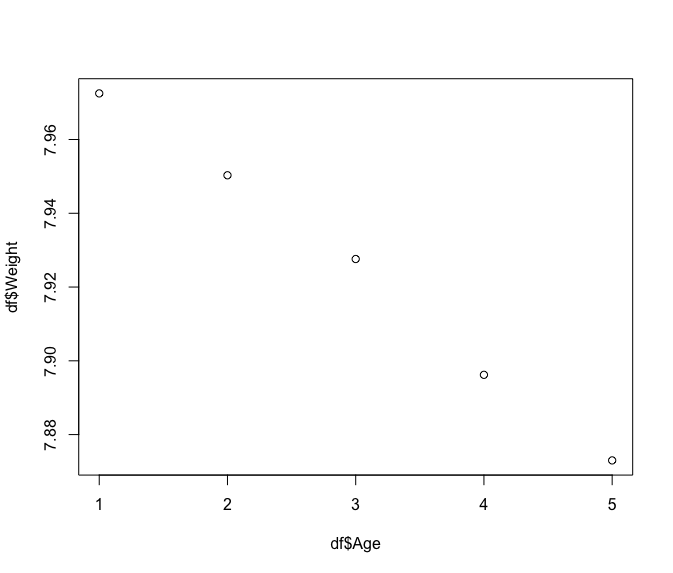
\includegraphics[width = \textwidth]{Rplot.png}
      \end{center}
    \end{figure}
    \begin{figure}[H]
      \begin{center}
      \caption{SD of Weight vs Age}
      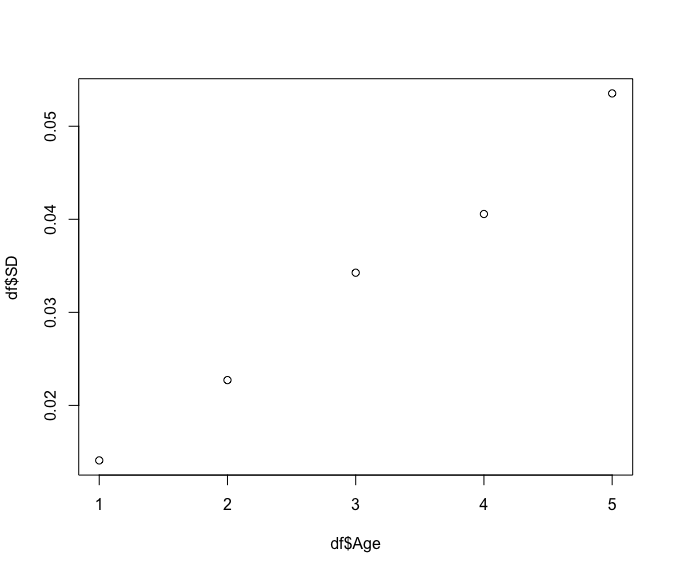
\includegraphics[width = \textwidth]{Rplot01.png}
      \end{center}
    \end{figure}
    \newpage

    \item[7.8.2] Fit a WLS regression with Weight as the response, using $Var(Weight|Age) = SD^2\sigma^2/n$ as the variance function. \\
    \solution Fitting the model in r we get the following, \\
     \textbf{Code:}
     \begin{center}
     \lstinputlisting[basicstyle = \small]{r1.txt}
     \end{center} 
  
       \begin{figure}[H] 
        \begin{center} 
        \caption{WLS model for Weight vs Age} 
        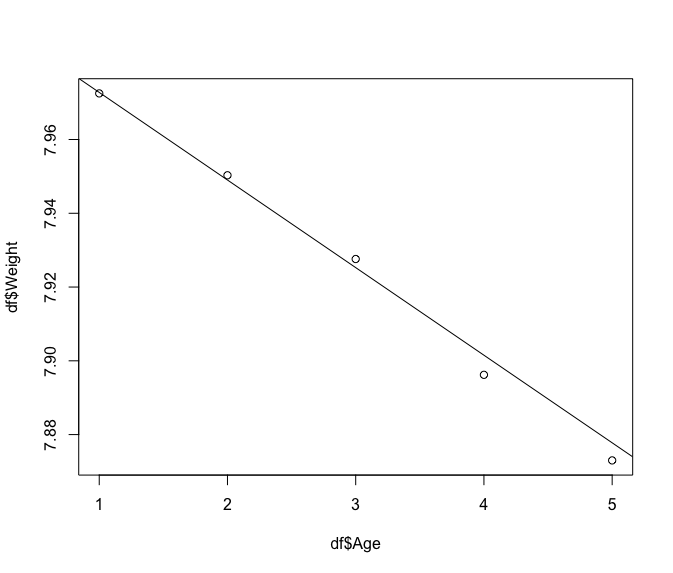
\includegraphics[width = \textwidth]{Rplot02.png} 
      \end{center} 
    \end{figure}
    \newpage

    \item[7.8.3] Is the fitted regression consistent with the known standard weight for a new coin.\\
    \solution The problem statement gives 7.9876g as the standard weight of a gold sovereign. We can see if our WLS regression is consistent by 
    computing the confidence interval on the intercept. Doing so we get, a 95 percent confidence interval of (7.99231466, 8.00072893) which excludes the 
    standard weight. I would see about experimenting with other weights especially since when we square the RSE we get a value around $1/4$ which goes against our assumption that 
    $\sigma^2 = 1$. \\
    \textbf{Code:}
    \begin{center}
    \lstinputlisting[basicstyle = \small]{r2.txt}
    \end{center} 
  \end{enumerate}
\end{exercise}
\newpage




\begin{exercise}{2} Use salarygov data. Although the response (MaxSalary) is a maximum of , rather than a mean of, sub-observations, fit the WLS model 
  with weight that represent rows' differing sample sizes. Your model should include the predictor Female\_dominated, the spline bases for Score, and the interaction terms 
  between these. A description of how to create Female\_dominated is given in 5.9.3. For the splines, use B-splines with 3 degrees of freedom. Once the model is fitted do the following:
  \begin{enumerate}
    \item[a.] Report the fitted model. \\
    \solution\\
    \textbf{Code:}
    \begin{center}
      \lstinputlisting[basicstyle = \small]{r3.txt}
      \end{center} 
      \newpage

    \item[b] Perform a partial F-test on the interaction terms to determine if female-dominated occupations require different spline coefficints than other occupations.\\
    \solution With a p-value of .00436 the following F-test tells us that female-dominated occupations require different spline coefficients.\\
    \textbf{Code:}
    \begin{center}
      \lstinputlisting[basicstyle = \small]{r4.txt}
      \end{center} 
      \newpage

      \item[c.] Give the residuals-vs-fitted values plot from the model that include the interaction terms and interpret the plot in terms of model assumptions. \\
      \solution  The residual plot seems to show some level of non-constant variance still. it does seem to be opening outwards ( like this"<") with a significant clustering towards 
      the initial values and around zero. Definitely does not look like random scatter. 
      
    \begin{figure}[H] 
      \begin{center} 
      \caption{Residual vs Fitted Plot} 
      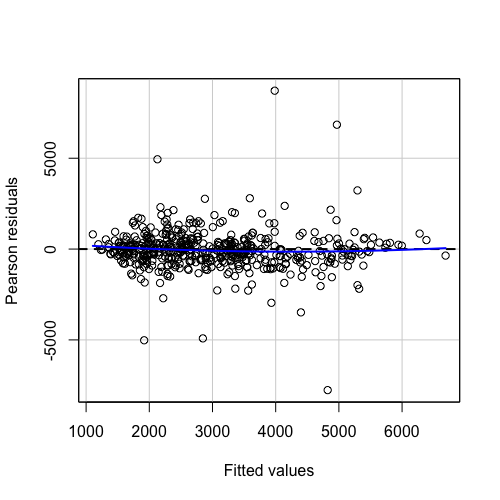
\includegraphics[width = \textwidth]{Rplot04.png} 
    \end{center} 
  \end{figure}
  \textbf{Code:}
  \begin{center}
    \lstinputlisting[basicstyle = \small]{r5.txt}
    \end{center} 


  \end{enumerate}

\end{exercise}
\newpage







\begin{exercise}{3.} The Blackmore data set in alr4 provides the number of hours of exercise performed each week by 236
  teenage girls at five different ages. It also provides a categorical indicator of whether the subject was hospitalized for an eating 
  disorder. Do the following, 
  \begin{enumerate}
    \item[a.] Fit a mixed model that controls for age and group as fixed effects and has a random intercept for subject. Give the estimated 
    variance component for subject and interpret it.\\
    \solution Fitting the mixed model with the lmer function we get a estimated variance component for subject of 3.898, a non-insignificant in the mean exercise score 
    and subjects. \\
    \textbf{Code:}
    \begin{center}
      \lstinputlisting{r6.txt}
      \end{center} 
    \newpage

    \item[b.] Test the variance component for subject is equal to 0 using a likelihood ratio test. Report a test statistic, p-value, and your conclusion.\\ 
    \solution Fitting the regular fixed model, which excludes the random intercept subject parameter, we get a chi squared test statistic of 184.26 with a p-value on the order of 
    $10^{-16}$ which means that the random intercept subject predictor is significant. \\
    \textbf{Code:}
    \begin{center}
      \lstinputlisting[basicstyle = \small]{r7.txt}
      \end{center} 
    \newpage

    \item[c.] Produce a normal probability plot of the predicted random effects for subject. Interpret the plot and what it says about your model.\\
    \solution  Producing the normal probability plot in r we can see that the random effects do not look to be normally distributed. We should not trust this model, and probably experiment with 
    other mixed models. 
    \begin{figure}[H] 
      \begin{center} 
      \caption{normal probability plot for predicted random effects.} 
      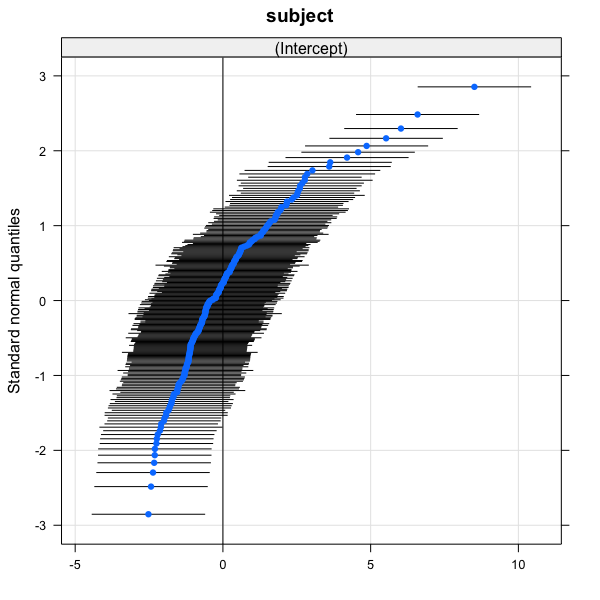
\includegraphics[width = \textwidth]{Rplot05.png} 
    \end{center} 
  \end{figure}
  \end{enumerate}
  
\end{exercise}





\end{document}





















